\begin{figure*}[t]
\centering
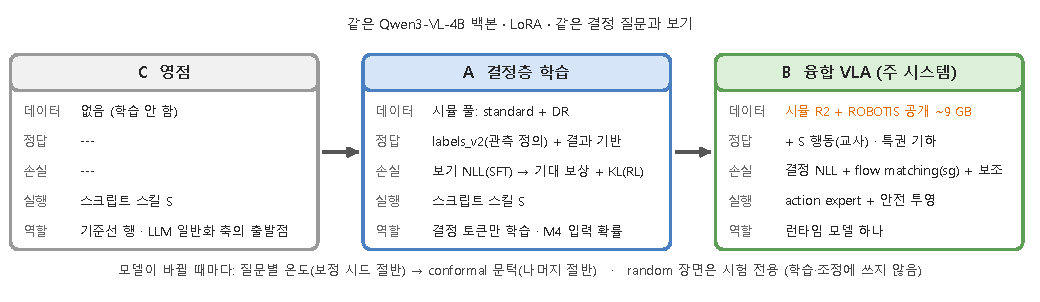
\includegraphics[width=\linewidth]{figures/training.pdf}
\caption{\textbf{학습 단계 C $\rightarrow$ A $\rightarrow$ B.} 같은 백본과 같은 결정 질문·보기를 유지한 채 학습량만 늘린다. C는 학습하지 않은 기준선이고, A는 결정 토큰만 관측 정의 정답(labels\_v2)과 결과 기반 보상으로 학습하며, B는 action expert(기울기 차단)와 보조 기하 헤드를 더한 주 시스템이다. 모델이 바뀔 때마다 보정을 다시 맞춘다. 공개 실물 데이터(ROBOTIS AI Worker 1,575편, \tentative{약 9\,GB}, 10\,Hz)는 소규모 시험(S-E2E)용이다.}
\label{fig:training}
\end{figure*}
